\subsection{Short term speckle pulsing}\label{short_pulse_sec}

To measure the PSD and the cutoff $k_c$ of the speckle potentials with short term speckle pulsing, we derive the evolution of the momentum states under two approximations. The first is the Raman-Nath approximation, atoms do not move far during the pulse.  The second is that the evolution time is short compared to $\hbar/V(x)$, so atoms do not acquire a phase comparable to $2\pi$.
Consider Hamiltonian
\begin{equation}
    \hat{H} = \frac{\hbar^2k^2}{2m} + V(x).
\end{equation}
The time evolution operator is
\begin{equation}
    \hat{U}(t) = \exp{-i\frac{\Delta t}{\hbar}\left[\frac{\hbar^2k^2}{2m}+V(x)\right]},
\end{equation}
Define $E_c$ as the energy associated with $k_c$, $\tau = \frac{\Delta t}{\hbar}E_c$, $\hat{k} = \frac{k}{k_c}$ and $S(x) = \frac{V(x)}{E_c}$
\begin{equation}
    \hat{U}(t) = \exp{-i\tau\left[\hat{k}^2+S(x)\right]}.
\end{equation}
Expand the operator to second order, 
\begin{equation}
    \hat{U}(t) = \exp{-i\tau\hat{k}^2/2}\exp{-i\tau S(x)}\exp{-i\tau\hat{k}^2/2}.
\end{equation}
We assume the initial state is $\ket{k=0}$, so the third term does not contribute. And we measure the distribution in $k$ space, so we can ignore the first term. The second term governs the short time evolution. To the lowest order, 
\begin{equation}
    \hat{U}(t)\ket{k=0} = \ket{k=0} - i\tau S(x) \ket{k=0}
\end{equation}
Expand $S(x)$ in $k$ space,
\begin{equation}
    S(x) = \sum_{k,k'}\Tilde{S}(k-k')\dyad{k}{k'}
\end{equation}
So
\begin{equation}
    \hat{U}(t)\ket{k=0} = \ket{k=0} - i\tau \sum_{\delta k}\Tilde{S}(\delta k)\ket{\delta k}
\end{equation}
The probability distribution of momentum states at time $\tau$ is
\begin{equation}\label{short_dist}
    P(k,\tau) = \tau^2 |\Tilde{S}(k)|^2 + \delta_{k,0}.
\end{equation}
It is proportional to the PSD of the speckle potential $|\Tilde{S}(k)|^2$ ignoring the central peak at $k=0$.

In the experiments, we put an iris right before the diffuser $D$ in \ref{fig:design}. By opening and closing the iris, we can control the size of the beam which determines $k_c$ of the speckle potential PSD in the focal plane. As the model we derived in Ch.~(\ref{speckle_chapter}) shows, the speckle beam size at the focal plane does not change with the beam size at the diffuser. The beam size at the focal plane is determined by the field-field correlation length at the diffuser. So the average speckle potential depth is proportional to the power of the beam which we can control when we change the size of the iris. 

We did the experiments for two iris sizes, $6.5\ {\rm mm}$ and $15\ {\rm mm}$, which correspond to $k_c=0.65k_r$ and $k_c=1.30k_r$, respectively. Here $k_r$ is defined with the largest recoil $k$ vector of atoms scattered by a $532\ {\rm nm}$ light beam focused by a one inch $f=30\ {\rm mm}$ lens. 
\begin{equation}
    k_r = \frac{2\pi}{532 {\rm nm}}\sin{\frac{\theta_{\rm R}}{2}}
\end{equation}
$\theta_{\rm R} \approx 45^\circ $ is shown in Fig.~(\ref{fig:raman_design}).
The average speckle potential match in both cases by controlling the power of the beam after the iris. 

We prepare BECs in a cross dipole trap, at $t=0$, we turn off the dipole trap and release the atoms for time-of-flight (TOF). Immediately after the dipole trap is turned off, we turn on the speckle beam and pulse for a short period of time, ranging from $20\ {\rm \mu s}$ to $250\ {\rm \mu s}$. After $18\ {\rm ms}$ TOF, we take absorption images of the atoms.

To compare with the experimental data, we simulate the process numerically. In the numerical simulation, we prepare the ground state of BECs in a dipole trap. At $t=0$, turn off the dipole trap and release the atoms. Immediately after, the speckle potential is turned on for a duration of $50\ {\rm \mu s}$ or $100\ {\rm \mu s}$, followed by free evolution for up to $20\ {\rm ms}$. We keep track of the momentum distribution of the atoms during the evolution. 

\begin{figure*}
    \centering
    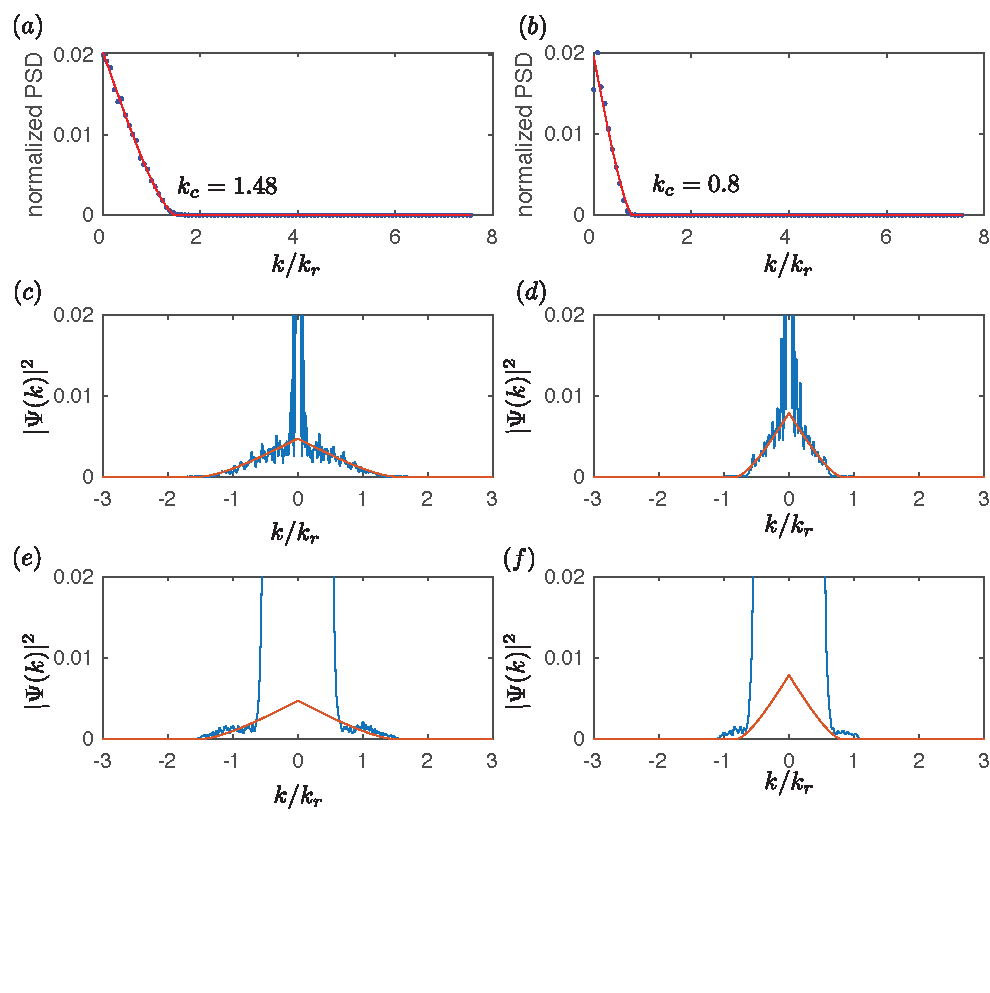
\includegraphics{Chapter6_secs/speckle_pulsing_simu.pdf}
    \caption{Simulation of short-term speckle pulsing. The left panel is for speckle potential with $k_c = 1.48k_r$, and the right panel for $k_c = 0.8k_r$. (a) and (b) verify the $k_c$ of both speckle potentials by plotting their PSD. (c) and (d) are the momentum distribution of atoms after released from the dipole trap and evolve under speckle pulses for $50\ {\rm \mu s}$. The red curves are proportional to the corresponding PSD of the speckle potential. The momentum distribution is an average of 20 speckle realizations. (e) and (f) are the momentum distribution of atoms after released from the dipole trap and evolve under speckle pulses for $50\ {\rm \mu s}$ followed by a $20\ {\rm ms}$ free expansion. The results are averaged over 20 speckle realizations. }
    \label{fig:speckle_pulsing_simu}
\end{figure*}

As Fig.~(\ref{fig:speckle_pulsing_simu}) shows, the simulation is done under two kinds of speckle potentials with different $k_c$ to compare with the experimental data. The left panel of Fig.~(\ref{fig:speckle_pulsing_simu}) is for the speckle potential with $k_c = 1.48k_r$ and the right panel for the speckle potential with $k_c = 0.80k_r$. Fig.~\ref{fig:speckle_pulsing_simu}(c) and Fig.~\ref{fig:speckle_pulsing_simu}(d) show the momentum distribution of atoms immediately after a $50\ {\rm \mu s}$ speckle pulsing, the results are averaged over 20 speckle realizations. The red curves are proportional to the PSD of the two kinds of speckle potentials, respectively. From Fig.~\ref{fig:speckle_pulsing_simu}(c) and Fig.~\ref{fig:speckle_pulsing_simu}(d) we can see the tail of the momentum distribution of atoms after short-term speckle pulsing matches with the PSD of the speckle potentials. The results agree with the analytical calculation of the momentum distribution in Eq.~(\ref{short_dist}), which predicts the momentum distribution to be a central $\delta$ function plus a tail that is proportional to the PSD of the speckle potentials. 

Fig.~\ref{fig:speckle_pulsing_simu}(e) and Fig.~\ref{fig:speckle_pulsing_simu}(f) show the momentum distribution of atoms after a $50\ {\rm \mu s}$ speckle pulse and a $20\ {\rm ms}$ time-of-flight (TOF). During the TOF, the mean-field expansion of the atoms broadens the momentum distribution. Both the central peak and the tail of the momentum distribution become broader after the TOF. In Fig.~\ref{fig:speckle_pulsing_simu}(f), for the speckle potential of smaller $k_c$, the tail of the momentum distribution is broadened more significantly. The broadened momentum distribution after TOF makes it harder to distinguish the speckle potentials with the tail of the momentum distribution.

\begin{figure*}
    \centering
    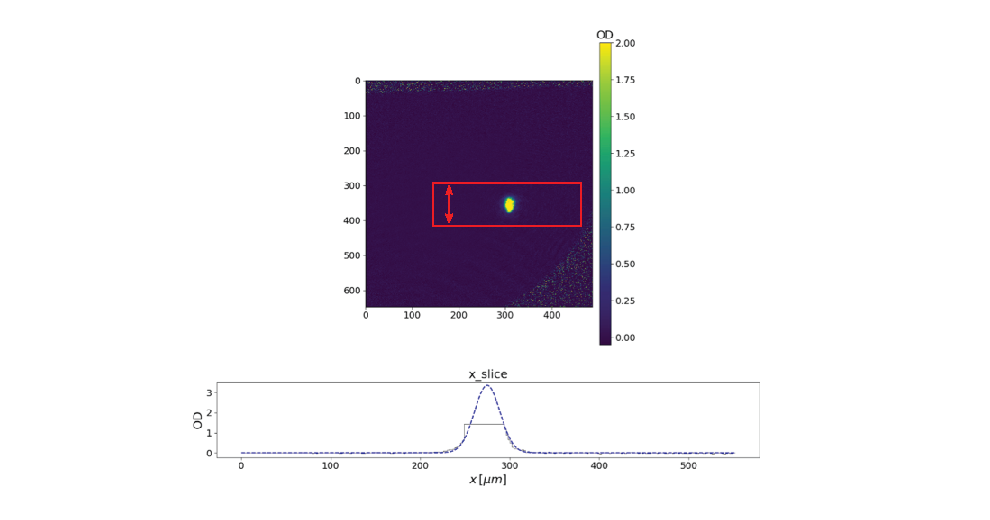
\includegraphics{Chapter6_secs/colOD.pdf}
    \caption{A sample of absorption images of atoms and analysis. The red square is a selected region of interest and the red arrow indicates the direction we take average. The masked and averaged spatial distribution of atoms (black curve) and a fitted Gaussian curve (blue dashed) are plotted below.}
    \label{fig:colOD}
\end{figure*}

\begin{figure*}
    \centering
    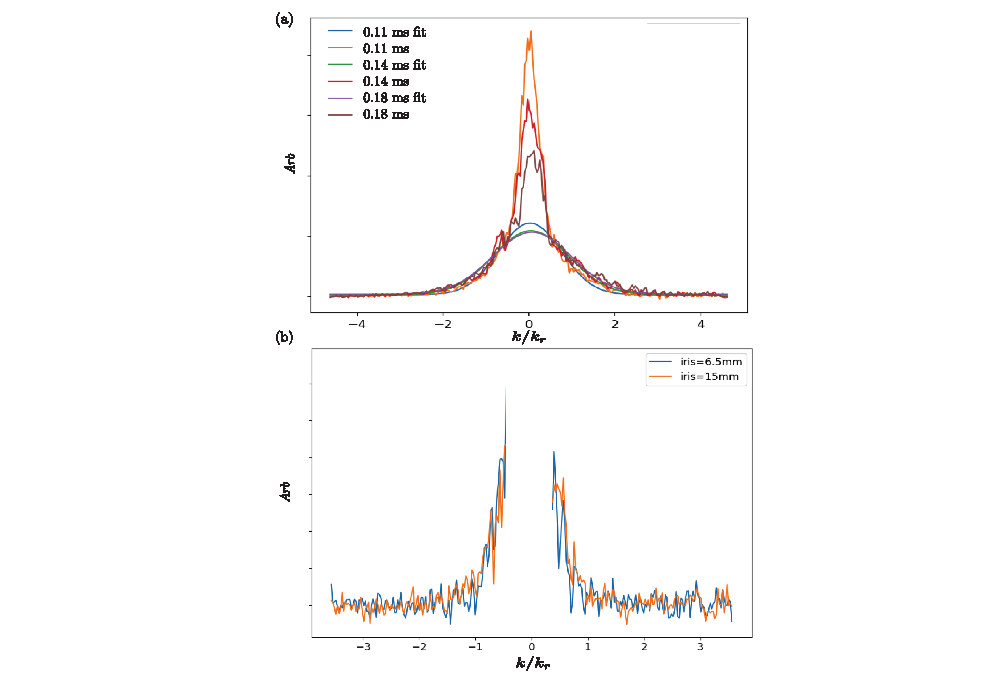
\includegraphics{Chapter6_secs/short_pulse.pdf}
    \caption{Momentum distribution after short-term speckle pulses and $18\ {\rm mm}$ TOF. (a). A few samples of momentum distribution of atoms without mask, along with fitted Gaussian curves to the masked momentum distribution. (b). The tails of the momentum distribution after short-term pulses of speckle potential with different PSD. The PSD of the speckle potentials are controlled by the iris sizes and the results are averaged for speckle pulsing time ranging from $80\ {\rm \mu s}$ to $150\ {\rm \mu s}$.}
    \label{fig:short_pulse}
\end{figure*}


Fig.~\ref{fig:colOD} and Fig.~\ref{fig:short_pulse} show the analysis results of the absorption images after TOF for two kinds of speckle potentials generated with different iris sizes. During TOF, the momentum distribution of atoms is mapped to their spatial distribution. From the absorption images, we can compute the momentum distribution from the spatial profile of the atoms. In the analysis, from the absorption images of atoms after TOF shown in Fig.~\ref{fig:colOD}, we select a region of interest around the center of the atoms indicated by the red square. And compute the average spatial distribution of atoms along the horizontal direction (red arrow). The central peak of this average spatial distribution is masked to show the detail of the tails. Fig.~\ref{fig:colOD} shows an example of the masked averaged spatial distribution along $x$ direction (black curve) and a Gaussian fit (blue dashed curve). The resultant tails of the spatial distribution are averaged over short-term speckle pulsing duration ranging from $80\ {\rm \mu s}$ to $150\ {\rm \mu s}$. The tails of the spatial distribution are then converted to that of the momentum distribution in a unit of $k_r$. 


Fig.~\ref{fig:short_pulse}(a) shows a few samples of the averaged momentum distribution along $x$ direction without a mask for short-term speckle pulsing, along with fitted Gaussian curves to the masked momentum distribution. From Fig.~\ref{fig:short_pulse}(a) we can see it is necessary to mask the central peak of the momentum distribution in order to analyze the width of the tails. Fig.~\ref{fig:short_pulse}(b) is the momentum distribution of atoms after short-term pulses of speckle potentials with different PSD, averaged over pulsing duration ranging from $80\ {\rm \mu s}$ to $150\ {\rm \mu s}$. From Fig.~\ref{fig:short_pulse}(b), it is hard to tell the difference between the two curves for two reasons. First, in the absorption images, the signal-noise-ratio at the tails of the density profile is low. Just by taking the average, it is hard to reduce the noise and see the clear tails as in the numerical simulation in Fig.~\ref{fig:speckle_pulsing_simu}. Second, as the simulation results show in Fig.~\ref{fig:speckle_pulsing_simu}(e) and Fig.~\ref{fig:speckle_pulsing_simu}(f), during TOF, the mean-field expansion broadens the momentum distribution more significantly for speckle pulsing with smaller $k_c$. So the width of the tails of the momentum distribution for the pulsing of two kinds of speckle potentials is closer to each other after TOF than before. For the two reasons, we conclude we can not quantitatively measure the $k_c$ of the speckle potential by using the absorption images after short-term speckle pulsing and TOF.


